% vim:spelllang=ru,en
\documentclass[a4paper,12pt,notitlepage,headsepline,pdftex]{scrartcl}

\usepackage{cmap} % чтобы работал поиск по PDF
\usepackage[T2A]{fontenc}
\usepackage[utf8]{inputenc}
\usepackage[english,russian]{babel}
\usepackage{concrete}
\usepackage{cite}
\usepackage{url}

\usepackage{textcase}
\usepackage[pdftex]{graphicx}

\usepackage{lscape}

\pdfcompresslevel=9 % сжимать PDF
\usepackage{pdflscape} % для возможности альбомного размещения некоторых страниц
\usepackage[pdftex]{hyperref}
% настройка ссылок в оглавлении для pdf формата
\hypersetup{unicode=true,
            pdftitle={ПОЭВМ Лаба №4},
            pdfauthor={Погода Михаил},
            pdfcreator={pdflatex},
            pdfsubject={},
            pdfborder    = {0 0 0},
            bookmarksopen,
            bookmarksnumbered,
            bookmarksopenlevel = 2,
            pdfkeywords={},
            colorlinks=true, % установка цвета ссылок в оглавлении
            citecolor=black,
            filecolor=black,
            linkcolor=black,
            urlcolor=blue}

\usepackage{amsmath}
\usepackage{amssymb}
\usepackage{moreverb}
\usepackage{indentfirst}
\usepackage{misccorr}

\usepackage{xtab}
\usepackage{nccfoots}
\usepackage{listings}

\lstloadlanguages{C++}
\lstset{language=C++,basicstyle=\scriptsize,frame=tb,commentstyle=\itshape,stringstyle=\bfseries,extendedchars=false}
\begin{document}
\begin{titlepage}
  \begin{center}
    \large
    \MakeUppercase{Министерство образования и науки,}

    \MakeUppercase{молодёжи и спорта Украины}

    \mbox{\MakeUppercase{Национальный технический университет Украины}}

    \MakeUppercase{,,Киевский политехнический институт''}

    \addvspace{6pt}

    \normalsize
    Кафедра прикладной математики

    \vfill

    \textbf{Отчёт}

    Лабораторная работа \No 4

    по дисциплине ,,Программное обеспечение ЭВМ''

    \emph{,,Методы безусловной оптимизации''}
  \end{center}

  \vfill

  \noindent
  \begin{minipage}{0.3\textwidth}
    Выполнил

    студент группы КМ-92

    Погода~М.\,В.
  \end{minipage}
  \hfill
  \begin{minipage}{0.4\textwidth}
    Проверила:

    Ковальчук"=Химюк~Л.\,А.
  \end{minipage}
  \vfill

  \begin{center}
    КИЕВ

    2012
  \end{center}
\end{titlepage}
\tableofcontents
\newpage
\section{Постановка задачи}
  Даны:
  \begin{itemize}
    \item Функция $f\left( \vec{x} \right)$
    \item Начальная точка: $\vec{x}_0$
  \end{itemize}

  Необходимо:
  \begin{itemize}
    \item найти локальный оптимум функции $f$ методом безусловной оптимизации;
    \item оценить точность полученного решения.
  \end{itemize}
\section{Входные данные}
  \hfill\emph{Вариант~11}

  \begin{itemize}
    \item \begin{equation}
        f\left( \vec{x} \right) = x_1^3 + x_2^3 - 3 x_1 x_2
        \label{eq:f}
      \end{equation}
    \item \begin{equation}
        \vec{x}_0 = \left( \begin{matrix}
          -1.0\\
          3.0
        \end{matrix}\right)
        \label{eq:x0}
      \end{equation}
  \end{itemize}

  В качестве метода безусловной оптимизации следует использовать метод
  Пауэлла.
  \newpage
\section{Теоретические сведения}
  В методе Пауэлла минимум функции $f\left( \vec{x} \right)$
  определяется путём проведения последовательных одномерных поисков, начиная с
  исходной точки $\vec{x}_0$ вдоль системы полученных сопряжённых направлений.

  Метод основан на теоретических результатах и используется для решения задач
  с квадратичными целевыми функциями.
  В окрестности точки минимума любую нелинейную функцию можно аппроксимировать
  квадратичной функцией.
  Работа алгоритма при решении задач с квадратичными функциями даёт
  представление о сходимости алгоритма, когда минимизируется функция общего
  вида.

  Квадратичная функция n независимых переменных, имеющая минимум, может быть
  минимизирована за n (или меньше) шагов, если шаги предпринимаются в
  сопряжённых направлениях.

  Алгоритм имеет вид:
  \begin{enumerate}
    \item Принять начальные направления $\vec{S}_1, \vec{S}_2, \dots, \vec{S}_n$ равными
      координатным осям.
    \item\label{en:p1} Произвести одномерный поиск из точки $\vec{x}_0$ вдоль направления
      $\vec{S}_n$.
      Полученную точку запомнить как $\vec{x}_1$.
    \item Произвести итеративную последовательность одномерных поисков,
      начиная из точки $\vec{x}_1$ вдоль направлений $\vec{S}_1, \vec{S}_2,
      \dots, \vec{S}_n$.
      Запомнить полученную точку как $\vec{x}_2$.
    \item Заменить $\vec{S}_1 \leftarrow \vec{S}_2, \vec{S}_2 \leftarrow
      \vec{S}_3, \dots \vec{S}_{n-1} \leftarrow \vec{S}_n$.
    \item Вычислить $\displaystyle \vec{S}_n = \frac{\vec{x}_2 -
      \vec{x}_1}{\left\|\vec{x}_2 - \vec{x}_1\right\|}$.
    \item Оценить критерий окончания метода:
      \begin{eqnarray}
        \left\| \vec{x_2} - \vec{x_1}\right\| < \varepsilon_x\\
        \left\| f\left( \vec{x_2} \right) - f\left( \vec{x_1} \right)
        \right\| < \varepsilon_f
        \label{eq:cr}
      \end{eqnarray}
    \item Если критерий не выполняется, то перейти на шаг~\ref{en:p1}
  \end{enumerate}
  \newpage
\section{Решение}


  \begin{table}[h]
    \centering
    \begin{tabular}{|c|c|c|}
      \hline
      $x_1$ & $x_2$ & $f\left( \vec{x} \right)$\\
      \hline
      $-1.0$ & $3.0$ & $33.0$\\
      $-1.0$ & $-\infty$ & $-\infty$\\
      \hline
    \end{tabular}
    \caption{Таблица промежуточных значений решения}
    \label{tab:tabs}
  \end{table}

\section{Описание программы}
  Программа написана на языке C++ с использованием библиотеки
  Qt\footnote{\url{http://qt-project.org}}.
  Программа ищет оптимум функции нескольких переменных методом сопряжённых
  направлений Пауэлла.

  Пользователь имеет возможность поменять начальную точку, а также начальный
  шаг одномерного поиска.

  В результате работы программы отображает все промежуточные точки полученные
  во время работы метода.
  Также вычисляется абсолютное отклонение полученной точки оптимума от
  теоретической точки оптимума функции, а также модуль разности функции в этих
  точках.
  \newpage
\section{Блок"=схема алгоритма}
  \begin{figure}[h!]
    \begin{center}
      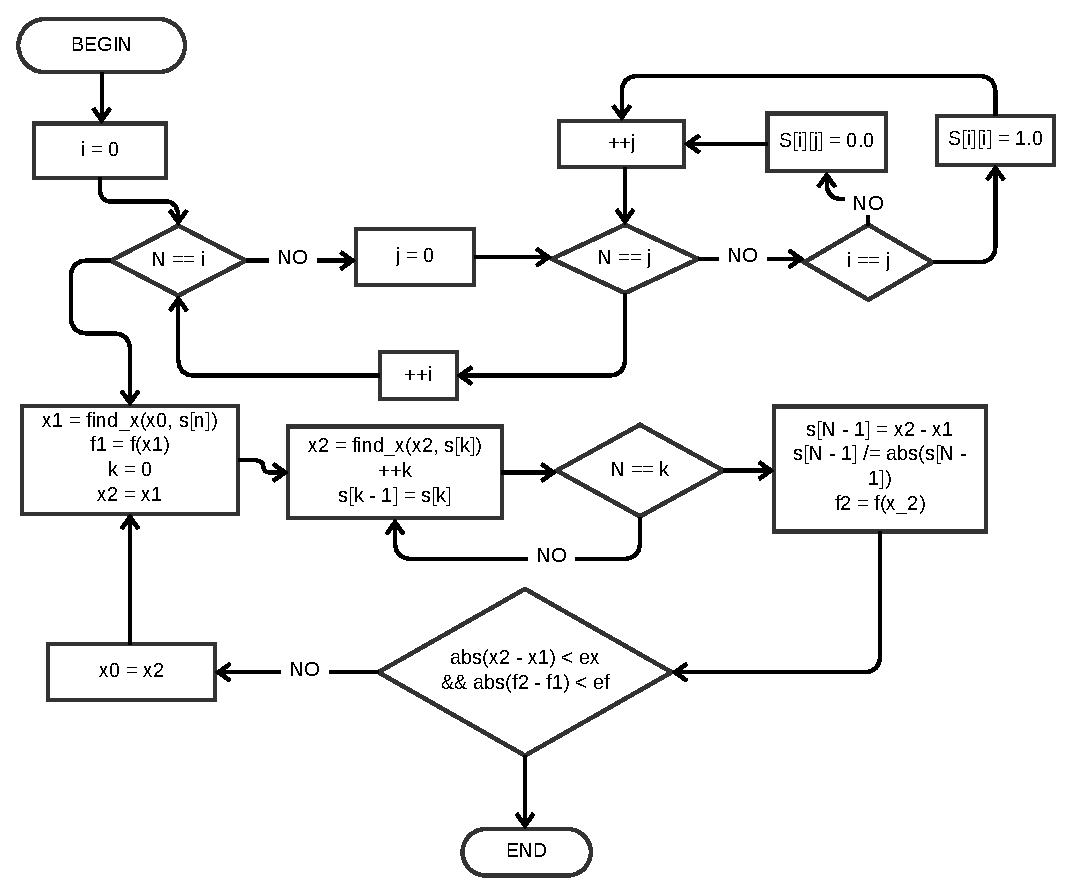
\includegraphics[scale=0.60]{flowchart.eps}
    \end{center}
    \caption{Блок"=схема алгоритма}
    \label{fig:flowchart}
  \end{figure}
  \newpage
\section{Выводы}
  При выполнении данной лабораторной работы был реализован метод безусловной
  оптимизации функции нескольких переменных, а также метод одномерного
  поиска, который используется в реализованном методе сопряжённых направлений
  Пауэлла.

  Метод Пауэлла имеет хорошую сходимость, если начальная точка находится
  вблизи локального минимума.

  Начальный вектор $\vec{x}_0$, заданный в условии, находится вне области
  локального минимума функции $f\left( \vec{x} \right)$, поэтому
  аппроксимация функции квадратичной функцией вносит существенную погрешность
  и метод стремится вдоль одного направления на бесконечность (т.\,к.
  глобального минимума у функции не существует).

  Однако, если принять $\displaystyle \vec{x}_0 = \left( \begin{matrix}
    0.8\\
    1.2
  \end{matrix}\right)$, метод сходится к точке локального оптимума ($x^\ast =
  \left( \begin{matrix}
    1.0\\
    1.0
  \end{matrix}\right)$), что видно на снимке экранной формы на
  странице~\pageref{fig:gui}
  \newpage
\section{Приложения}
  \subsection{Графическая форма приложения}
    \begin{figure}[h!]
      \begin{center}
        \includegraphics[scale=0.86]{scr.png}
      \end{center}
      \caption{Графическая форма приложения}
      \label{fig:gui}
    \end{figure}
  \subsection{Исходные тексты}
    \subsubsection{CMakeLists.txt}
      \lstinputlisting{/home/projects/apps-for-computing/lab4/CMakeLists.txt}
    \subsubsection{lab4\_widget.hxx}
      \lstinputlisting{/home/projects/apps-for-computing/lab4/lab4_widget.hxx}
    \subsubsection{lab4\_widget.cxx}
      \lstinputlisting{/home/projects/apps-for-computing/lab4/lab4_widget.cxx}
\end{document}
